%!TEX root = ProgCPP_ZF.tex

\part{Exceptions ("`Ausnahmen"')}

\section{Exception vs. Error}
Bitte unterscheiden Sie zwischen Exception (Ausnahme) und Error (Fehler)\\
\begin{itemize}
	\item \textbf{Error (Fehler):} Abweichung zur Spezifikation ($"$falsch implementiert$"$). Errors sollten bei der Verifikation (Testen) entdeckt werden.
	\item \textbf{Exception (Ausnahme):} abnormale (aber vorhersehbare und mögliche) Bedingung bei der Programmausführung.
	\item Wir sprechen hier über Exception Handling (der Ausdruck Error Handling ist aus oben genannten Gründen eigentlich falsch, obwohl er sehr häufig verwendet wird). Leider heissen auch die Standardklassen in C++ häufig xyz\_error statt xyz\_exception (schade, ist nicht einmal konsistent)
\end{itemize}

\section{Mögliche Reaktionen auf Ausnahmen}
\begin{itemize}
	\item \textbf{Ignorieren}\\
		Motto: $"$Augen zu und durch$"$ Eine sehr risikoreiche Variante!
	\item \textbf{Programmabbruch}\\
		Merkt immerhin, dass etwas nicht in Ordnung ist, die Reaktion ist aber unbefriedigend. Ist Exception Detection aber nicht eigentlich Exception Handling.
	\item \textbf{Exceptioncodes} (nicht Fehlercodes)\\
		Funktionen geben als Rückgabewert, als Parameter oder global einen Ausnahmecode an.
\end{itemize}

\subsection{Exceptioncodes als Rückgabewert}
\begin{multicols}{2}
\begin{minipage}{\linewidth}
\vspace{-2\baselineskip}
\begin{lstlisting}
if (eOk == s.push(elem))
{
	...
}
else
{
	... // handle exception
}
\end{lstlisting}
\end{minipage}
\vfill\null
\columnbreak
\begin{itemize}
	\item Rückgabewert wird von Exceptioncodes belegt (ist unschön)
	\item Geht nicht bei Konstruktoren (Ctors haben keinen Rückgabewert)
	\item Bei differenzierten Exceptioncodes gibt es stark verschachtelte if ... else bei jedem Aufruf $\rightarrow$ unleserlich
\end{itemize}
\end{multicols}

\subsection{Exceptioncodes als Referenzparameter}
\begin{multicols}{2}
\begin{minipage}{\linewidth}
	\vspace{-2\baselineskip}
\begin{lstlisting}
s.push(elem, excpt);
if (eOk == excpt)
{
	...
}
else
{
	... // handle exception
}
\end{lstlisting}
\end{minipage}
\vfill\null
\columnbreak
\begin{itemize}
	\item Aufruf wird mit zusätzlichem Referenzparameter für den Exceptioncode erweitert (ist unschön)
	\item Bei differenzierten Exceptioncodes gibt es stark verschachtelte if ... else bei jedem Aufruf $\rightarrow$ unleserlich	
\end{itemize}
\end{multicols}
\vfill
\pagebreak\newpage

\subsection{Globaler Exceptioncode}
\begin{multicols}{2}
\begin{minipage}{\linewidth}
\vspace{-2\baselineskip}
\begin{lstlisting}
s.push(elem);	// globalException is set
if (eOk == globalException)
{
	...
}
else
{
	... // handle Exception
}
\end{lstlisting}	
\end{minipage}
\vfill\null
\columnbreak
\begin{itemize}
	\item Führt aufgrund des globalen Exceptioncodes zu schwer les- und wartbaren Programmen.
	\item Bei differenzierten Exceptioncodes gibt es stark verschachtelte if ... else bei jedem Aufruf $\rightarrow$ unleserlich
\end{itemize}
\end{multicols}

\subsection{Wo sollen Exceptions behandelt werden?}
\begin{itemize}
	\item Fact: Exceptions können irgendwo im Programm entstehen
	\item Wie soll auf Exceptions reagiert werden?
	\item Eine angemessene Reaktion kann häufig nicht ausschliesslich an der Stelle des Auftretens gemacht werden
	\item Die Reaktion muss auch weiter $"$nach oben$"$ gereicht werden können, bis auf die Applikationsebene, wo allenfalls eine Mitteilung an den Benutzer getätigt wird.
	\item[\-] \begin{hinweis}
		Grundsatz: Nur das regeln, was sinnvoll ist und auf einer bestimmten Stufe wirklich entschieden werden kann, sonst nach oben weiterreichen.
	\end{hinweis}
\end{itemize}

\section{Ziel für Exception Handling}
\begin{itemize}
	\item $"$Normaler$"$ Programmablauf (Schönwetterfall) wird durch das Exception Handling nicht tangiert
	\item Der Normalfall soll einfach gelesen werden können
	\item Der Ausnahmefall ist klar und einfach geregelt
	\item Der Overhead soll möglichst klein sein
	\item Die Weiterreichung an die nächsthöhere Funktion im Call Stack soll einfach sein
\end{itemize}

\section{Exception Handling in C++}
\begin{itemize}
	\item Exceptions werden in Form eines Objekts am Ort ihres Auftretens ausgeworfen (explizit oder auch $"$automatisch$"$) (werfen = to throw)
	\item Exception Handler versuchen, diese Exception-Objekte aufzufangen (to catch)
\end{itemize}

\subsection{Exception Handling in C++: Syntax}
\begin{minipage}{\linewidth}
\vspace{-\baselineskip}
\begin{lstlisting}
try
{
	... // Code, der eine Exception auswerfen koennte
}
catch (const MyExceptionClass& exc)
{
	... // wenn ein Objekt der Klasse MyExceptionClass oder einer Unterklasse
			// davon ausgeworfen wurde, dann kann dieser Handler das Objekt fangen
}

// u.U. weitere Catches
\end{lstlisting}
\end{minipage}
\vfill
\pagebreak\newpage

\subsection{Auslösen (Werfen) von Ausnahmen}
\begin{itemize}
	\item Ausnahmen können mit dem Schlüsselwort \emph{throw} explizit ausgeworfen werden
	\item Nach einem \emph{throw-}Befehl wird das Programm abgebrochen und beim ersten passenden umgebenden Handler fortgesetzt
	\item Dabei werden alle lokalen Objekte wieder automatisch zerstört (Stack unwinding)
	\item Geworfen werden kann ein beliebiges Objekt (üblich: ein spezifisches C++-Ausnahmeobjekt)
	\item (Ausschliesslich) innerhalb eines Exception Handlers ist auch die Form\hspace{0.05\linewidth}
	\begin{minipage}{0.1\linewidth}
	\vspace{-\baselineskip}
\begin{lstlisting}
throw;
\end{lstlisting}
	\end{minipage}\\
	erlaubt. Dadurch wird die Exception an den nächsten Handler weitergereicht (Exception propagation).
\end{itemize}

\subsubsection{Beispiel für Exception Handling: unübliche Variante}
\vspace{-\baselineskip}
\begin{multicols}{2}
\begin{minipage}{\linewidth}
\begin{lstlisting}
class Xcpt
{
	public:
		Xcpt(const char* text);
		~Xcpt();
		const char* getDiagStr() const;
	private:
		const char* diagStr;
};

void allocateFoo()
{
	b1();
	if (0 == allocation())
		throw Xcpt("Allocation failed!");
	b2();
}
\end{lstlisting}
\end{minipage}
\begin{minipage}{\linewidth}
\begin{lstlisting}
// Testprogramm
void testFoo()
{
	a1();
	try
	{
		a2();
		allocateFoo();
		a3();
	}
	catch (const Xcpt& exc)
	{
		cout << "Caught exception. Text: " << exc.getDiagStr() << endl;
	}
	a4();
}
\end{lstlisting}
\end{minipage}
\end{multicols}

\begin{multicols}{2}
\subsection{Vordefinierte Ausnahmeklassen}
\begin{itemize}
	\item Ausnahmeobjekte können beliebigen Typs sein (z.B. auch \emph{int}). Meist werden jedoch spezifische hierarchisch organisierte C++-Ausnahmeklassen verwendet.
	\item Vordefinierte Standardklasse: \emph{exception}
\end{itemize}
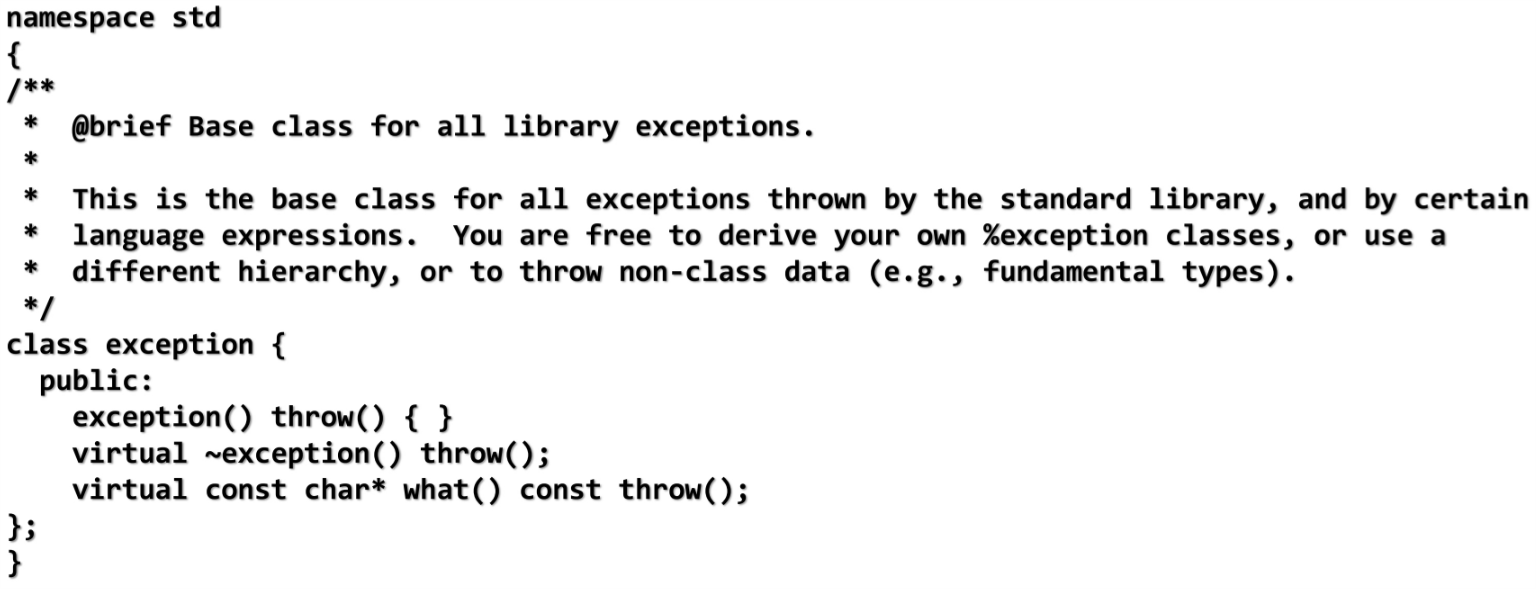
\includegraphics[width=\linewidth]{images/exceptionClass.png}
\end{multicols}

\begin{multicols}{2}
\subsection{Exception-Hierarchie in C++}
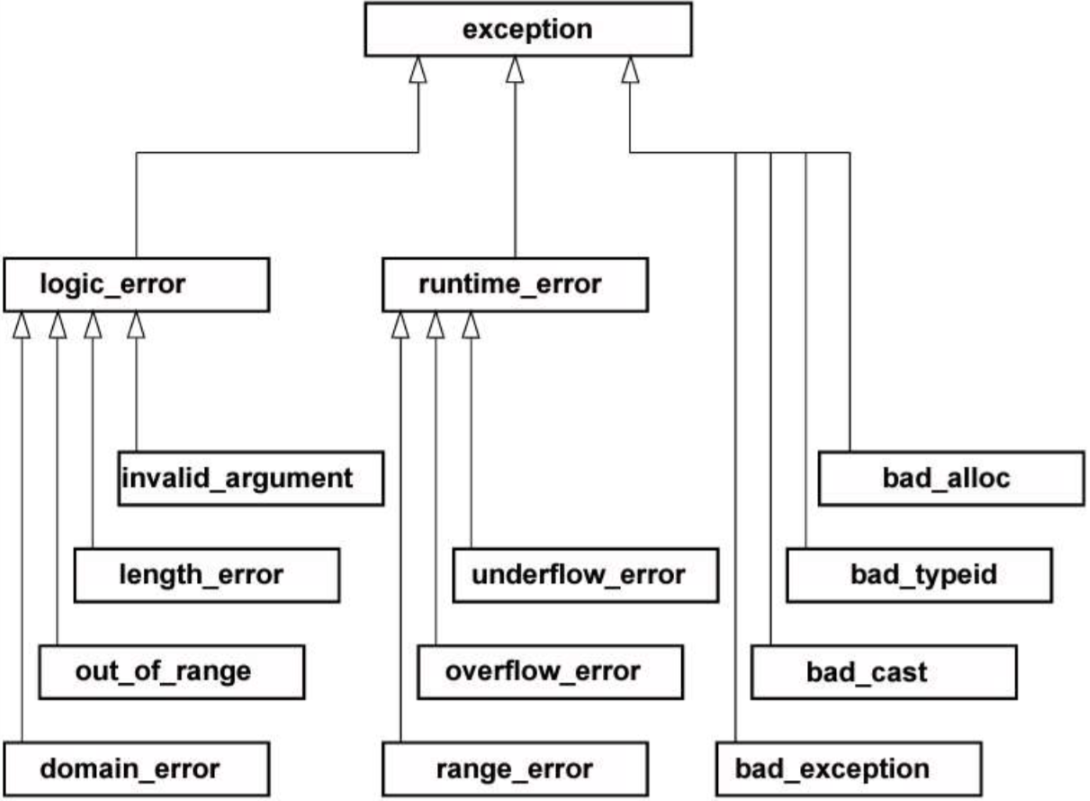
\includegraphics[width=0.8\linewidth]{images/exceptionHierarchie.png}
\vfill\null
\columnbreak
\subsection{Laufzeit- vs. Logische "`Fehler"'}
\begin{itemize}
	\item Logische "Fehler" (logic\_error)
	\begin{itemize}
		\item Ausnahmen im Programmablauf, die bereits zur Entwicklungszeit ihre Ursachen haben.
		\item Theoretisch könnten diese Ausnahmen verhindert werden.
	\end{itemize}
	\item Laufzeit"fehler" (runtime\_error)
	\begin{itemize}
		\item Nicht vorhersehbare Ausnahmen wie z.B. arithmetische Überläufe
		\item Diese Ausnahmen treten erst zur Laufzeit auf, z.B. durch eine nicht erlaubte Benutzereingabe
	\end{itemize}
\end{itemize}
\end{multicols}

\begin{multicols}{2}
\subsection{Exceptions und ihre Header-Dateien}
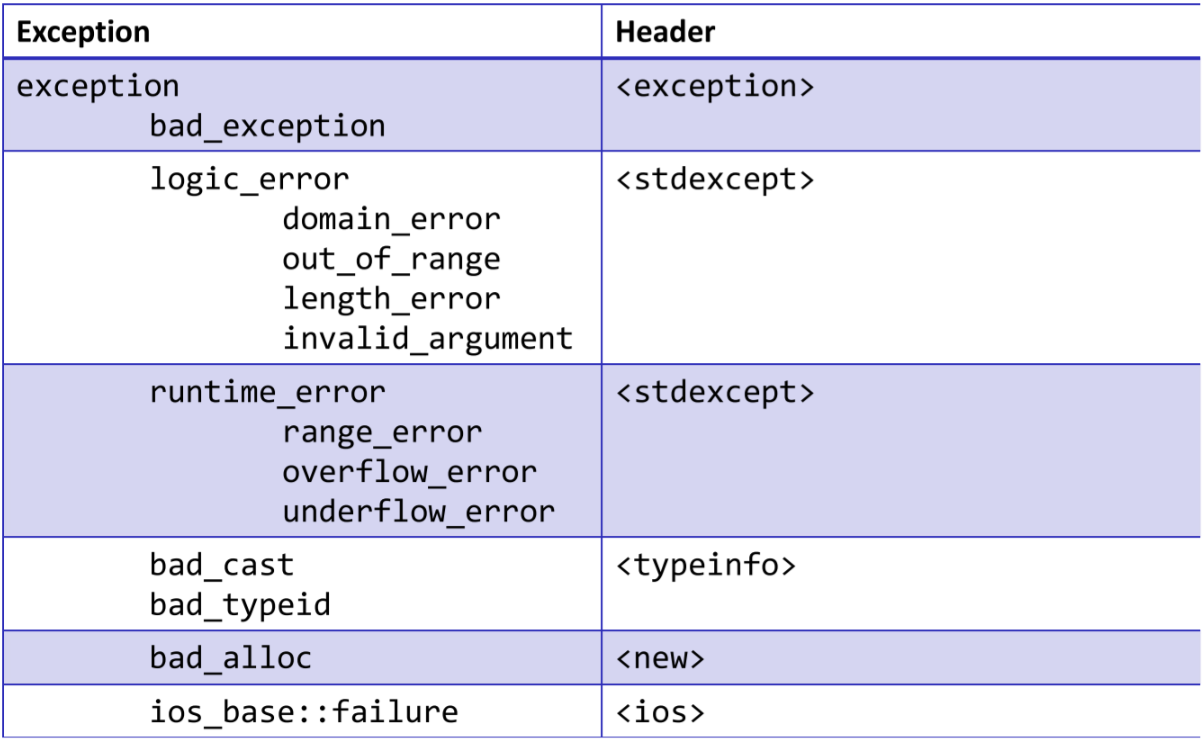
\includegraphics[width=\linewidth]{images/exceptionHeader.png}
\vfill\null
\columnbreak
\subsection{Exception Handler}
\begin{itemize}
	\item Ein oder mehrere Exception Handler können hintereinander definiert werden
	\item Die einzelnen \emph{catch}-Handler müssen sich in den Parametern unterscheiden
	\item Wenn eine Exception geflogen kommt, wird \textbf{der erste passende Handler} genommen. Ein passender Handler macht ein \emph{catch} auf genau diese Exception oder auf eine Basisklasse derselben.
	\item[\-] \begin{achtung}
	Deshalb (\textbf{sehr wichtig}): Der allgemeinste Handler (am weitesten oben in der Hierarchie) muss der letzte \emph{catch}-Handler sein.
	\end{achtung}
\end{itemize}
\end{multicols}

\subsection{Exception Handler 2}
\begin{itemize}
	\item Wenn kein Handler passt, dann wird im Aufrufstack nach oben gesucht, ob ein passender Handler vorhanden ist.
	\item Wenn auch dort keiner gefunden wird, dann wird die Funktion \emph{terminate()} aufgerufen.
	\item \emph{terminate()} beendet das Programm, kann aber auch selbst definiert werden.
	\item Catch all\\
	Der folgende Handler fängt ausnahmslos alle Exceptions ab (und muss wenn gewünscht deshalb immer als letzter aufgeführt werden):\hspace{0.05\linewidth}
	\begin{minipage}{0.15\linewidth}
	\vspace{-\baselineskip}
\begin{lstlisting}
catch(...) {}
\end{lstlisting}
	\end{minipage}
\end{itemize}

\subsection{Exception Propagation}
\begin{itemize}
	\item Innerhalb eines Exception Handlers kann eine Exception mittels\\
	\textbf{throw;}\\
	weitergereicht werden.
	\item Die Exceptiion wird dann auch nicht etwa an das nächste \textbf{catch(...)} weitergeleitet, sondern an die aufrufende Funktion.
\end{itemize}

\subsection{Exception Specification}
\begin{minipage}{0.6\linewidth}
\vspace{-\baselineskip}
\begin{lstlisting}
void foo() throw(/* Liste der Exceptions */);
\end{lstlisting}
\end{minipage}
\begin{itemize}
	\item Die Liste spezifiziert, welche Exceptions von einem Aufrufer von \emph{foo()} erwartet werden müssen.
	\item Aber: garantiert auch, dass das Programm abstürzt, wenn eine andere als eine der spezifizierten Exceptions ausgeworfen wird, d.h. \emph{foo()} muss dafür sorgen, dass wirklich nur die aufgelisteten Exceptions ausgeworfen werden.
	\item Genauer: falls eine nicht spezifizierte Exception ausgeworfen wird, dann wird die Funktion \emph{unexpected()} aufgerufen, welche üblicherweise das Programm abbricht.
	\item \emph{unexpected()} kann selbst definiert werden.
\end{itemize}
\vfill
\pagebreak\newpage

\subsubsection{Exception Specification: Beispiele}
\begin{minipage}{0.7\linewidth}
\vspace{-\baselineskip}
\begin{lstlisting}
void foo1() throw(specificXcpt1, specificXcpt2);
// die zwei angegebenen Exceptions muessen vom Aufrufer von
// foo1() erwartet werden.

void foo2() throw();
// KEINE Exceptions koennen geflogen kommen

void foo3();
// beliebige Exceptions muessen erwartet werden
\end{lstlisting}
\end{minipage}

\subsubsection{Exception Handling in der Praxis}
\begin{itemize}
	\item Exceptions sollen nur für Ausnahmen, nicht für den normalen Ablauf verwendet werden
	\item Exceptions sollen nicht vorbeugende Abfragen ersetzen
	\item Ein Programm soll nur gegen $"$entscheidende$"$ Ausnahmen abgesichert werden
	\item Wenn eine Exception ausgeworfen wird, dann wird normalerweise eine der vordefinierten Exceptionklassen oder eine (evtl. selbst definierte) Unterklasse davon genommen
	\item Exception specifications werden, wenn überhaupt, nur bei ausgewählten (Schnittstellen-)Funktionen definiert
	\item \textbf{Always throw exceptions by value, and catch them by const reference.}
\end{itemize}

\subsubsection{Handling von System Exceptions}
\begin{multicols}{2}
\begin{minipage}{\linewidth}
\vspace{-\baselineskip}
\begin{lstlisting}
int Calculator::divide()
{
	if (0 == nr2)
		throw runtime\_error("Division durch Null");
	
	return nr1 / nr2;
}
\end{lstlisting}
\end{minipage}
\vfill\null
\columnbreak
Q: In obiger Variante wird verhindert, dass überhaupt erst eine Division durch Null ausgeführt wird. Könnte die Division nicht einfach probiert werden? Das System sollte ja wenn nötig eine Runtime Exception selbständig auswerfen?
\begin{minipage}{\linewidth}
\vspace{-\baselineskip}
\begin{lstlisting}
int Calculator::divide()
{
	return nr1 / nr2;
}
\end{lstlisting}
\end{minipage}
\end{multicols}

\subsubsection{Betreibt meine Umgebung Exception Mapping?}
\begin{itemize}
	\item Mit Hilfe des folgenden Codeausschnitts kann einfach überprüft werden, ob eine bestimmte Umgebung Exception Mapping betreibt:
	\begin{minipage}{\linewidth}
	\vspace{-\baselineskip}
\begin{lstlisting}
try
{
	int a = 5;
	int b = a/0;
}
catch (...)
{
	cout << "Caught exception if exception is mapped" << endl;
}
\end{lstlisting}
	\end{minipage}
	\item Unter Umständen muss die Null über \emph{cin} (zur Laufzeit) eingegeben werden, da $"$freundliche$"$ Compiler allenfalls darauf hinweisen, dass eine Division durch Null nicht geht.
\end{itemize}